\hypertarget{libthinkpad_8h}{
\section{libthinkpad.h File Reference}
\label{libthinkpad_8h}\index{libthinkpad.h@{libthinkpad.h}}
}




This graph shows which files directly or indirectly include this file:\nopagebreak
\begin{figure}[H]
\begin{center}
\leavevmode
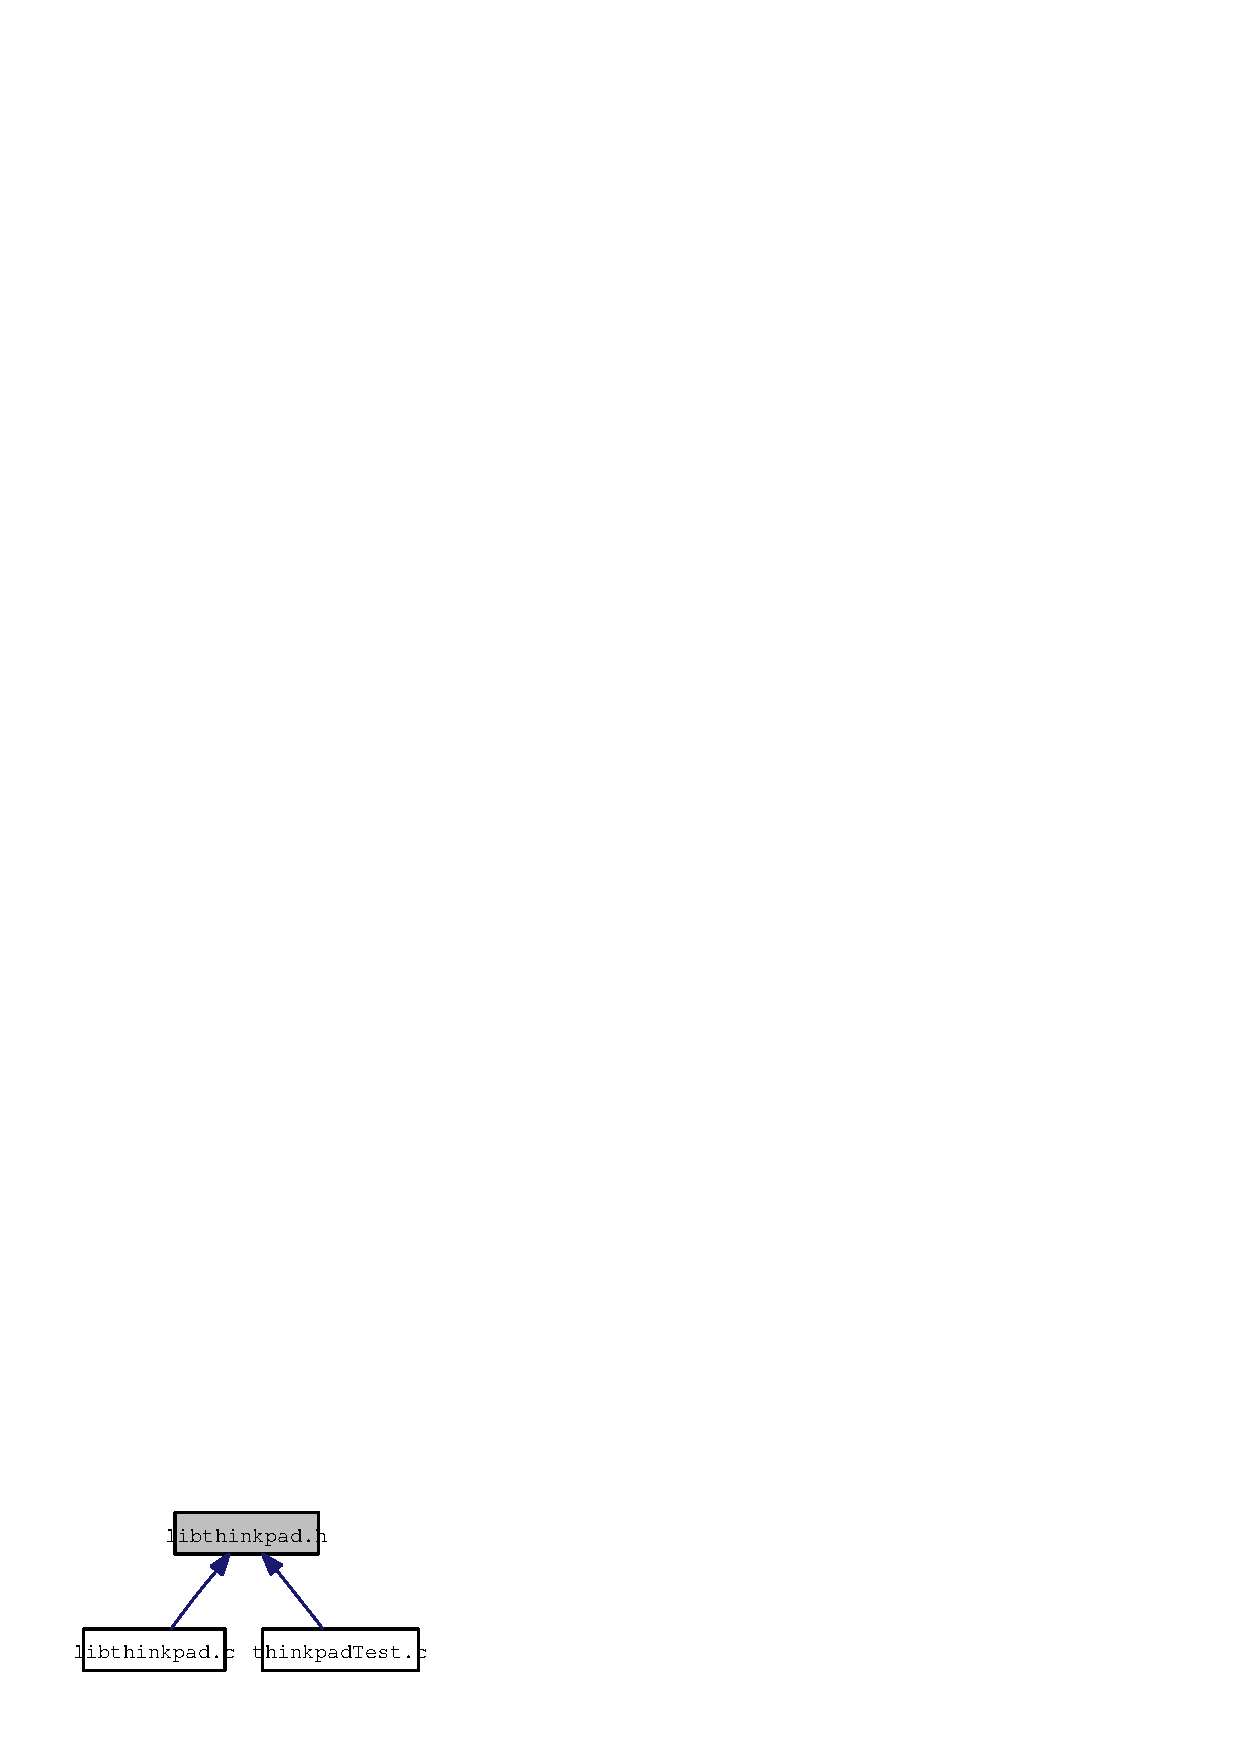
\includegraphics[width=102pt]{libthinkpad_8h__dep__incl}
\end{center}
\end{figure}
\subsection*{Defines}
\begin{CompactItemize}
\item 
\#define \hyperlink{libthinkpad_8h_4c0cbefe7ca00462bb109b7968fe272d}{LIGHTPROC}~\char`\"{}/proc/acpi/ibm/light\char`\"{}
\end{CompactItemize}
\subsection*{Functions}
\begin{CompactItemize}
\item 
int \hyperlink{libthinkpad_8h_90f318656de4ddfd918141e20059474b}{blinkLight} (int on, int off, int num)
\item 
int \hyperlink{libthinkpad_8h_1c8a5a0db5fb813f149d4145c7d4a475}{blinkMorseChar} (char c)
\item 
int \hyperlink{libthinkpad_8h_f42de626f64ff9ca399eb971d8cd07c1}{blinkMorseString} (char $\ast$c)
\end{CompactItemize}


\subsection{Define Documentation}
\hypertarget{libthinkpad_8h_4c0cbefe7ca00462bb109b7968fe272d}{
\index{libthinkpad.h@{libthinkpad.h}!LIGHTPROC@{LIGHTPROC}}
\index{LIGHTPROC@{LIGHTPROC}!libthinkpad.h@{libthinkpad.h}}
\subsubsection{\setlength{\rightskip}{0pt plus 5cm}\#define LIGHTPROC~\char`\"{}/proc/acpi/ibm/light\char`\"{}}}
\label{libthinkpad_8h_4c0cbefe7ca00462bb109b7968fe272d}




Definition at line 22 of file libthinkpad.h.

Referenced by blinkLight(), and help\_\-function().

\subsection{Function Documentation}
\hypertarget{libthinkpad_8h_90f318656de4ddfd918141e20059474b}{
\index{libthinkpad.h@{libthinkpad.h}!blinkLight@{blinkLight}}
\index{blinkLight@{blinkLight}!libthinkpad.h@{libthinkpad.h}}
\subsubsection{\setlength{\rightskip}{0pt plus 5cm}int blinkLight (int {\em on}, int {\em off}, int {\em num})}}
\label{libthinkpad_8h_90f318656de4ddfd918141e20059474b}


Switch the light over the lcd on and off (blinking).

\begin{Desc}
\item[Parameters:]
\begin{description}
\item[{\em on}]The time how long the light is switched on \item[{\em off}]The time how long the light is switched off \item[{\em num}]How often the light switching between on and off\end{description}
\end{Desc}
\begin{Desc}
\item[Returns:]The return value is 0 if all is okay or -1 if they was an error \end{Desc}


Definition at line 50 of file libthinkpad.c.

References LIGHTPROC.

Referenced by main().

Here is the caller graph for this function:\nopagebreak
\begin{figure}[H]
\begin{center}
\leavevmode
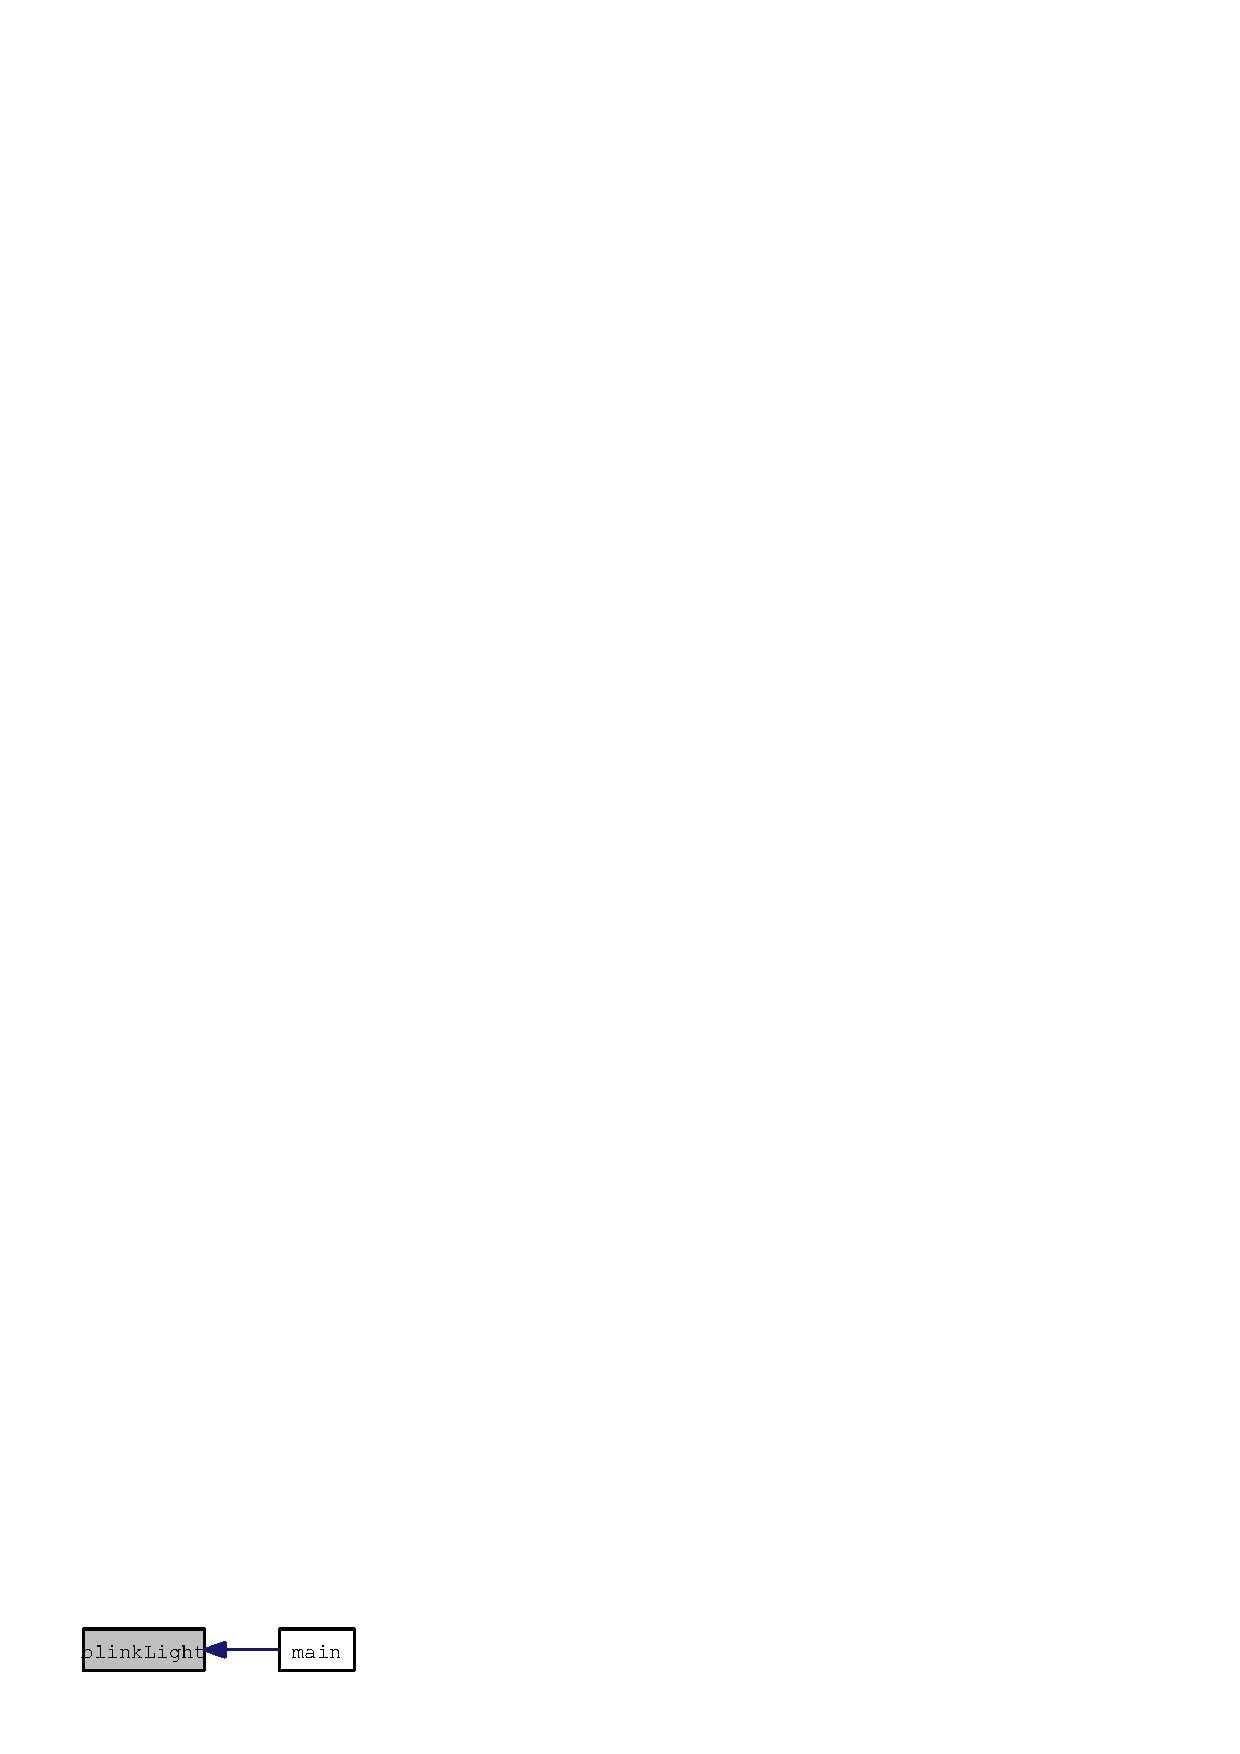
\includegraphics[width=87pt]{libthinkpad_8h_90f318656de4ddfd918141e20059474b_icgraph}
\end{center}
\end{figure}
\hypertarget{libthinkpad_8h_1c8a5a0db5fb813f149d4145c7d4a475}{
\index{libthinkpad.h@{libthinkpad.h}!blinkMorseChar@{blinkMorseChar}}
\index{blinkMorseChar@{blinkMorseChar}!libthinkpad.h@{libthinkpad.h}}
\subsubsection{\setlength{\rightskip}{0pt plus 5cm}int blinkMorseChar (char {\em c})}}
\label{libthinkpad_8h_1c8a5a0db5fb813f149d4145c7d4a475}


This function takes a char, and blinks than the letter in morsecode. \hyperlink{structMorsecode}{Morsecode} (\char`\"{}.\char`\"{} = short alias point, \char`\"{}-\char`\"{} = long alias line):

a -$>$ .- n -$>$ -. b -$>$ -... o -$>$ --- c -$>$ -.-. p -$>$ .--. d -$>$ -.. q -$>$ --.- e -$>$ . r -$>$ .-. f -$>$ ..-. s -$>$ ... g -$>$ --. t -$>$ - h -$>$ .... u -$>$ ..- i -$>$ .. v -$>$ ...- j -$>$ .--- w -$>$ .-- k -$>$ -.- x -$>$ -..- l -$>$ .-.. y -$>$ -.-- m -$>$ -- z -$>$ --..

1 -$>$ .---- 6 -$>$ -.... 2 -$>$ ..--- 7 -$>$ --... 3 -$>$ ...-- 8 -$>$ ---.. 4 -$>$ ....- 9 -$>$ ----. 5 -$>$ ..... 0 -$>$ -----

\begin{Desc}
\item[Parameters:]
\begin{description}
\item[{\em c}]The char for the morsecode\end{description}
\end{Desc}
\begin{Desc}
\item[Returns:]int The return value is 0 if all is okay or -1 if they was an error \end{Desc}


Definition at line 75 of file libthinkpad.c.

References Morsecode::line, morsecode, MORSLINE, MORSPOINT, Morsecode::pause, Morsecode::pausechar, Morsecode::pauseword, and Morsecode::point.

Referenced by blinkMorseString(), and main().

Here is the caller graph for this function:\nopagebreak
\begin{figure}[H]
\begin{center}
\leavevmode
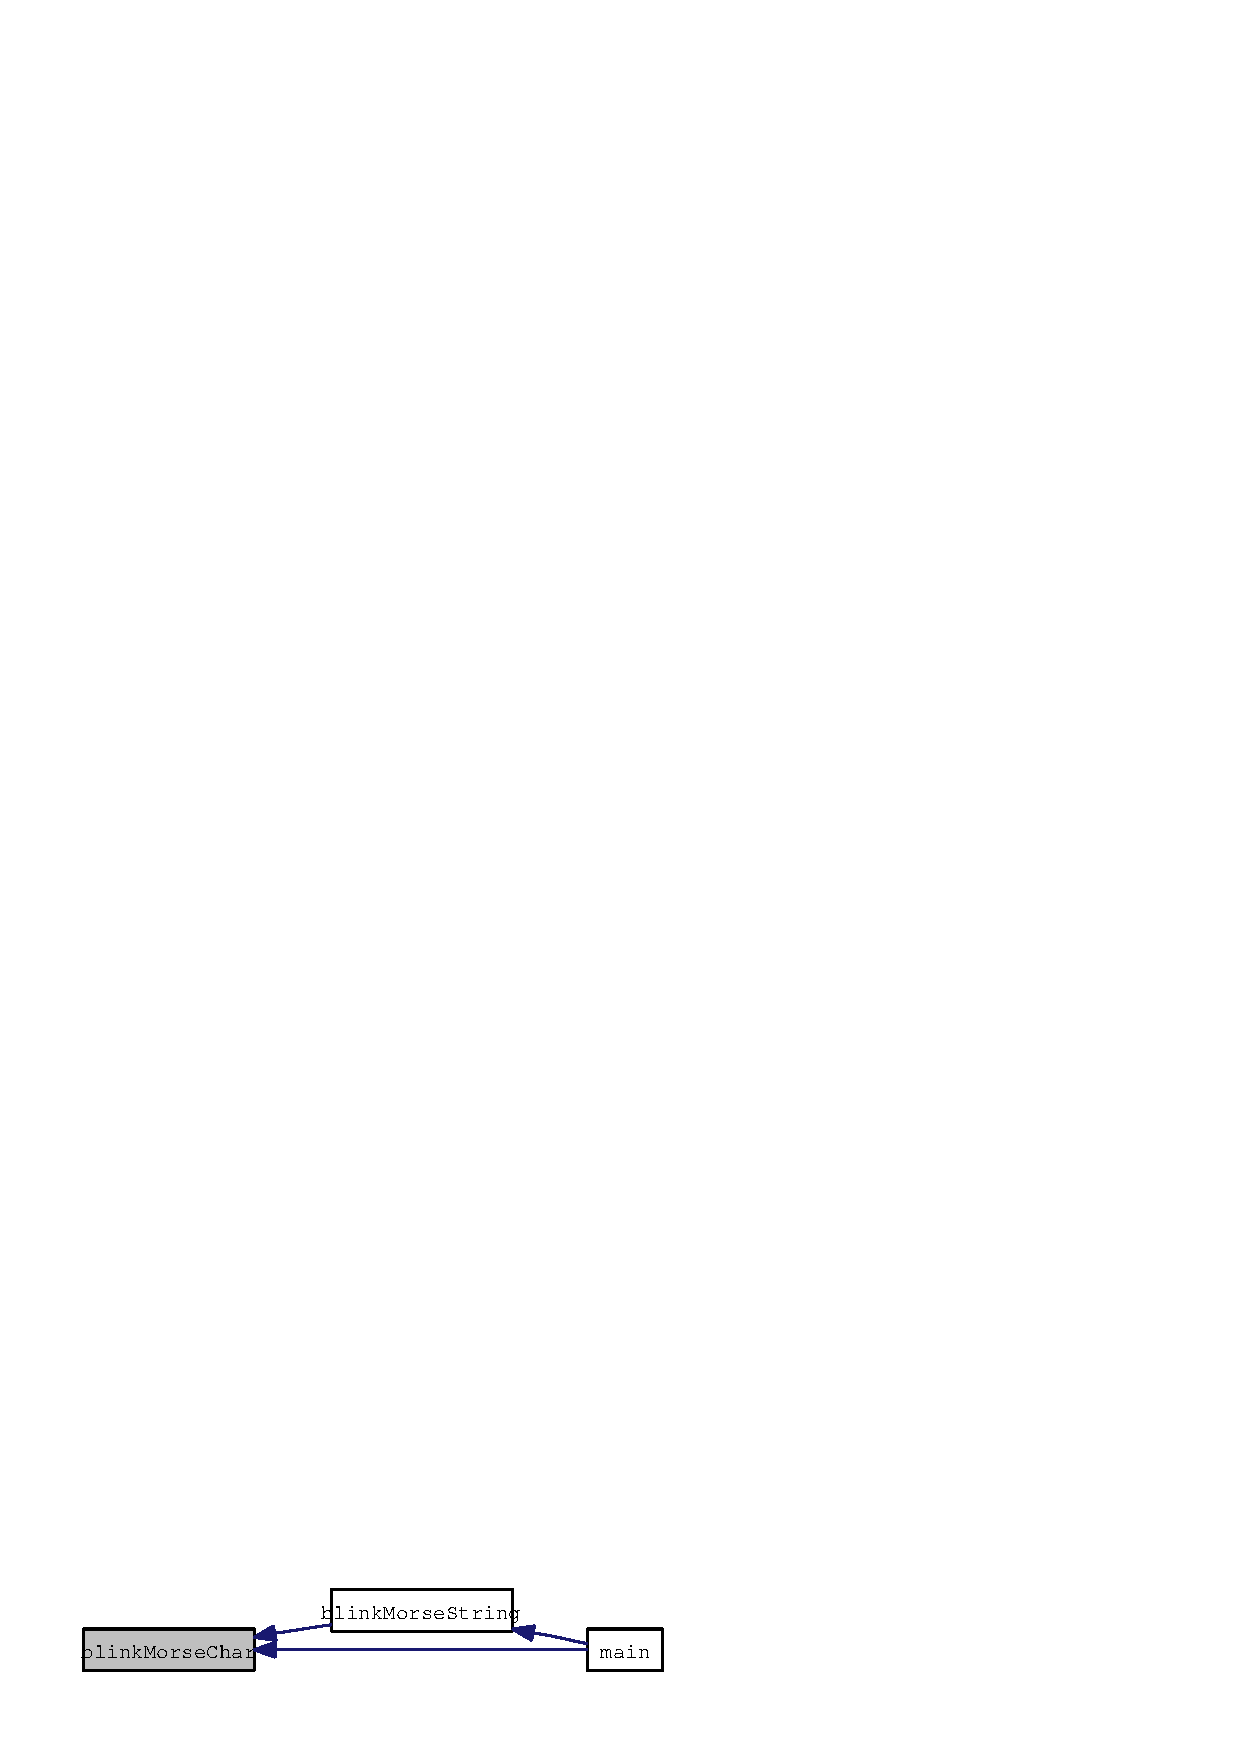
\includegraphics[width=161pt]{libthinkpad_8h_1c8a5a0db5fb813f149d4145c7d4a475_icgraph}
\end{center}
\end{figure}
\hypertarget{libthinkpad_8h_f42de626f64ff9ca399eb971d8cd07c1}{
\index{libthinkpad.h@{libthinkpad.h}!blinkMorseString@{blinkMorseString}}
\index{blinkMorseString@{blinkMorseString}!libthinkpad.h@{libthinkpad.h}}
\subsubsection{\setlength{\rightskip}{0pt plus 5cm}int blinkMorseString (char $\ast$ {\em c})}}
\label{libthinkpad_8h_f42de626f64ff9ca399eb971d8cd07c1}


